\documentclass[journal, a4paper]{IEEEtran}

% some very useful LaTeX packages include:

%\usepackage{cite}      % Written by Donald Arseneau
                        % V1.6 and later of IEEEtran pre-defines the format
                        % of the cite.sty package \cite{} output to follow
                        % that of IEEE. Loading the cite package will
                        % result in citation numbers being automatically
                        % sorted and properly "ranged". i.e.,
                        % [1], [9], [2], [7], [5], [6]
                        % (without using cite.sty)
                        % will become:
                        % [1], [2], [5]--[7], [9] (using cite.sty)
                        % cite.sty's \cite will automatically add leading
                        % space, if needed. Use cite.sty's noadjust option
                        % (cite.sty V3.8 and later) if you want to turn this
                        % off. cite.sty is already installed on most LaTeX
                        % systems. The latest version can be obtained at:
                        % http://www.ctan.org/tex-archive/macros/latex/contrib/supported/cite/

\usepackage{graphicx}   % Written by David Carlisle and Sebastian Rahtz
                        % Required if you want graphics, photos, etc.
                        % graphicx.sty is already installed on most LaTeX
                        % systems. The latest version and documentation can
                        % be obtained at:
                        % http://www.ctan.org/tex-archive/macros/latex/required/graphics/
                        % Another good source of documentation is "Using
                        % Imported Graphics in LaTeX2e" by Keith Reckdahl
                        % which can be found as esplatex.ps and epslatex.pdf
                        % at: http://www.ctan.org/tex-archive/info/

%\usepackage{psfrag}    % Written by Craig Barratt, Michael C. Grant,
                        % and David Carlisle
                        % This package allows you to substitute LaTeX
                        % commands for text in imported EPS graphic files.
                        % In this way, LaTeX symbols can be placed into
                        % graphics that have been generated by other
                        % applications. You must use latex->dvips->ps2pdf
                        % workflow (not direct pdf output from pdflatex) if
                        % you wish to use this capability because it works
                        % via some PostScript tricks. Alternatively, the
                        % graphics could be processed as separate files via
                        % psfrag and dvips, then converted to PDF for
                        % inclusion in the main file which uses pdflatex.
                        % Docs are in "The PSfrag System" by Michael C. Grant
                        % and David Carlisle. There is also some information
                        % about using psfrag in "Using Imported Graphics in
                        % LaTeX2e" by Keith Reckdahl which documents the
                        % graphicx package (see above). The psfrag package
                        % and documentation can be obtained at:
                        % http://www.ctan.org/tex-archive/macros/latex/contrib/supported/psfrag/

%\usepackage{subfigure} % Written by Steven Douglas Cochran
                        % This package makes it easy to put subfigures
                        % in your figures. i.e., "figure 1a and 1b"
                        % Docs are in "Using Imported Graphics in LaTeX2e"
                        % by Keith Reckdahl which also documents the graphicx
                        % package (see above). subfigure.sty is already
                        % installed on most LaTeX systems. The latest version
                        % and documentation can be obtained at:
                        % http://www.ctan.org/tex-archive/macros/latex/contrib/supported/subfigure/

\usepackage{url}        % Written by Donald Arseneau
                        % Provides better support for handling and breaking
                        % URLs. url.sty is already installed on most LaTeX
                        % systems. The latest version can be obtained at:
                        % http://www.ctan.org/tex-archive/macros/latex/contrib/other/misc/
                        % Read the url.sty source comments for usage information.

%\usepackage{stfloats}  % Written by Sigitas Tolusis
                        % Gives LaTeX2e the ability to do double column
                        % floats at the bottom of the page as well as the top.
                        % (e.g., "\begin{figure*}[!b]" is not normally
                        % possible in LaTeX2e). This is an invasive package
                        % which rewrites many portions of the LaTeX2e output
                        % routines. It may not work with other packages that
                        % modify the LaTeX2e output routine and/or with other
                        % versions of LaTeX. The latest version and
                        % documentation can be obtained at:
                        % http://www.ctan.org/tex-archive/macros/latex/contrib/supported/sttools/
                        % Documentation is contained in the stfloats.sty
                        % comments as well as in the presfull.pdf file.
                        % Do not use the stfloats baselinefloat ability as
                        % IEEE does not allow \baselineskip to stretch.
                        % Authors submitting work to the IEEE should note
                        % that IEEE rarely uses double column equations and
                        % that authors should try to avoid such use.
                        % Do not be tempted to use the cuted.sty or
                        % midfloat.sty package (by the same author) as IEEE
                        % does not format its papers in such ways.

\usepackage{amsmath}    % From the American Mathematical Society
                        % A popular package that provides many helpful commands
                        % for dealing with mathematics. Note that the AMSmath
                        % package sets \interdisplaylinepenalty to 10000 thus
                        % preventing page breaks from occurring within multiline
                        % equations. Use:
%\interdisplaylinepenalty=2500
                        % after loading amsmath to restore such page breaks
                        % as IEEEtran.cls normally does. amsmath.sty is already
                        % installed on most LaTeX systems. The latest version
                        % and documentation can be obtained at:
                        % http://www.ctan.org/tex-archive/macros/latex/required/amslatex/math/



% Other popular packages for formatting tables and equations include:

%\usepackage{array}
% Frank Mittelbach's and David Carlisle's array.sty which improves the
% LaTeX2e array and tabular environments to provide better appearances and
% additional user controls. array.sty is already installed on most systems.
% The latest version and documentation can be obtained at:
% http://www.ctan.org/tex-archive/macros/latex/required/tools/

% V1.6 of IEEEtran contains the IEEEeqnarray family of commands that can
% be used to generate multiline equations as well as matrices, tables, etc.

% Also of notable interest:
% Scott Pakin's eqparbox package for creating (automatically sized) equal
% width boxes. Available:
% http://www.ctan.org/tex-archive/macros/latex/contrib/supported/eqparbox/

% *** Do not adjust lengths that control margins, column widths, etc. ***
% *** Do not use packages that alter fonts (such as pslatex).         ***
% There should be no need to do such things with IEEEtran.cls V1.6 and later.


% Your document starts here!
\begin{document}
\begin{titlepage}

\newcommand{\HRule}{\rule{\linewidth}{0.5mm}} % Defines a new command for the horizontal lines, change thickness here

\center % Center everything on the page
 %----------------------------------------------------------------------------------------
%	LOGO SECTION
%----------------------------------------------------------------------------------------

~\\[1cm]

\includegraphics{SCUT.png}\\[2cm] % Include a department/university logo - this will require the graphicx package

%----------------------------------------------------------------------------------------
%	TITLE SECTION
%----------------------------------------------------------------------------------------

\HRule \\[1cm]
{ \huge \bfseries The Experiment Report of \textit{Machine Learning} }\\[0.6cm] % Title of your document
\HRule \\[2cm]
%----------------------------------------------------------------------------------------
%	HEADING SECTIONS
%----------------------------------------------------------------------------------------


\textsc{\LARGE \textbf{School:} School of Software Engineering}\\[1cm]
\textsc{\LARGE \textbf{Subject:} Software Engineering}\\[2cm]


%----------------------------------------------------------------------------------------
%	AUTHOR SECTION
%----------------------------------------------------------------------------------------

\begin{minipage}{0.4\textwidth}
\begin{flushleft} \large
\emph{Author:}\\
Haipeng Deng % Your name
\end{flushleft}
\end{minipage}
~
\begin{minipage}{0.4\textwidth}
\begin{flushright} \large
\emph{Supervisor:} \\
Mingkui Tan % Supervisor's Name
\end{flushright}
\end{minipage}\\[2cm]
~
\begin{minipage}{0.4\textwidth}
\begin{flushleft} \large
\emph{Student ID:}\\
201730686193
\end{flushleft}
\end{minipage}
~
\begin{minipage}{0.4\textwidth}
\begin{flushright} \large
\emph{Grade:} \\
Undergraduate
\end{flushright}
\end{minipage}\\[2cm]

% If you don't want a supervisor, uncomment the two lines below and remove the section above
%\Large \emph{Author:}\\
%John \textsc{Smith}\\[3cm] % Your name

%----------------------------------------------------------------------------------------
%	DATE SECTION
%----------------------------------------------------------------------------------------

{\large \today}\\[2cm] % Date, change the \today to a set date if you want to be precise


%----------------------------------------------------------------------------------------

\vfill % Fill the rest of the page with whitespace

\end{titlepage}

% Define document title and author
	\title{Lab 1 : Linear Regression and Stochastic Gradient Descent}
	\maketitle

% Write abstract here
\begin{abstract}
This report introduces my work in Lab 1 : Linear Regression and Stochastic Gradient Descent, where I constructed a linear regression model and implemented two basic methods of optimization i.e. closed-formed solution and stochastic gradient descent.
\end{abstract}

% Each section begins with a \section{title} command
\section{Introduction}
	% \PARstart{}{} creates a tall first letter for this first paragraph
\PARstart{L}{inear} regression, closed-formed solution and stochastic gradient descent are three fundamental concepts in machine learning. Although linear regression may seemed quite too simple compared to those complicated state-of-the-art models. It has been a readily comprehensible model for a machine learning starter. This lab is conducted in order to further understand the three concepts, conduct some experiments under small scale dataset, realize the process of optimization and adjusting parameters.

% Main Part
\section{Methods and Theory}
Simple linear regression describes the linear relationship between a variable, plotted on the x-axis, and a response variable y, plotted on the y-axis \\
\begin{figure}[!hbt]
		% Center the figure.
		\centering
		% Include the eps file, scale it such that it's width equals the column width. You can also put width=8cm for example...
		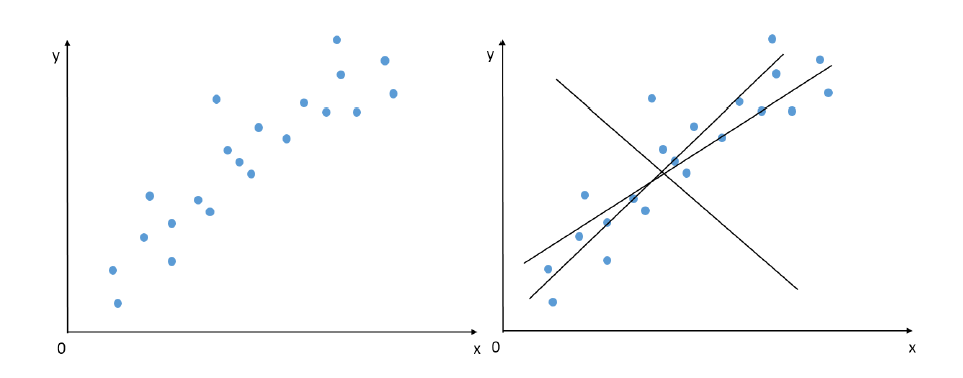
\includegraphics[width=\columnwidth]{linearRe.png}
		% Create a subtitle for the figure.
		\caption{Simple linear 1D regression}
		% Define the label of the figure. It's good to use 'fig:title', so you know that the label belongs to a figure.
		\label{fig1}
\end{figure}

The model function of linear regression is shown below:
\begin{align*}
f(x;b,w) &= b + w_1x_1 + ... + w_m x_m \\
&= \sum_{j=1}^mw_j x_j + b \\
&= w^Tx + b
\end{align*}

In this experiment, the least squared loss function is chosen to judge the "quality" of the model:
\begin{align*}
L_D(w) &= \frac1 2 \sum_{i=1}^n (y_i - f(x_i;w))^2\\
&= \frac1 2 \sum_{i=1}^n (y_i - \hat y_i)^2
\end{align*}

In closed-form solution, we directly derive the w* by analytical methods i.e. letting $ \frac{\partial L(w)}{\partial w} = -X^Ty + X^TXw = 0$.\\
And finally we can get $ w*=  (X^TX)^-1X^Ty$

In stochastic gradient descent method, after the loss function is chosen, a random sample will be selected to calculate the gradient of the model.
\begin{equation}
Gradient = \frac{\partial L(w)}{\partial w} = -X^Ty + X^TXw
\end{equation} 
We then optimize the linear model by adjusting w via following the opposite direction of the gradient. In this procedure, a hyperparameter $\eta$ will be set manually to control the "learning rate" of the descent process. The process can be described as:
\begin{equation}
w' \rightarrow w - \eta \frac{\partial L(w)}{\partial w}
\end{equation}

\section{Experiments}
\subsection{Dataset}
The dataset used in the experiment is "Housing" in LIBSVM Data, including 506 samples and each sample has 13 features. The dataset is split into a training set and a validation set as testing set is not required in this lab. The training set contains $ \frac23 $ of the whole dataset and the remaining data is used to examine how good is the model(validation set).

\subsection{Implementation}
In closed-form solution, I firstly initialize the training set and validation set using python method, write the code of deriving w* and the code of computing loss of the model. Then I finished this part by directly invoking the functions i wrote, which is quite simple.
\begin{figure}[!hbt]
		% Center the figure.
		\centering
		% Include the eps file, scale it such that it's width equals the column width. You can also put width=8cm for example...
		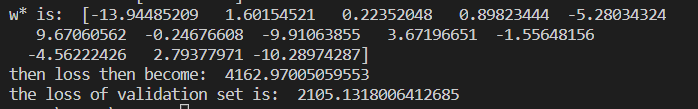
\includegraphics[width=\columnwidth]{closed-form.png}
		% Create a subtitle for the figure.
		\caption{result of closed-form solution}
		% Define the label of the figure. It's good to use 'fig:title', so you know that the label belongs to a figure.
		\label{fig2}
\end{figure}\\

In stochastic gradient descent method, I firstly split the dataset using the same strategy above. Then I initialize my model parameters w by setting all parameters into 0. After checking the original loss of my model, I start to randomly choose a sample in my dataset and compute its gradient corresponding to the loss function. The following step is to update my w by applying $ W_t = W_{t+1} + \eta D $ and compute the new loss. The two step above is conducted several times to observe how stochastic gradient descent helps optimize the model.\par
	% If you have questions about how to write mathematical formulas in LaTeX, please read a LaTeX book or the 'Not So Short Introduction to LaTeX': tobi.oetiker.ch/lshort/lshort.pdf

	% This is how you include a eps figure in your document. LaTeX only accepts EPS or TIFF files.
	\begin{figure}[!hbt]
		% Center the figure.
		\begin{center}
		% Include the eps file, scale it such that it's width equals the column width. You can also put width=8cm for example...
		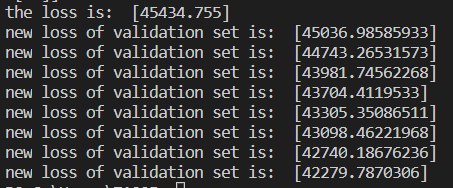
\includegraphics[width=\columnwidth]{sto.png}
		% Create a subtitle for the figure.
		\caption{Code output of stochastic gradient descent}
		% Define the label of the figure. It's good to use 'fig:title', so you know that the label belongs to a figure.
		\label{fig3}
		\end{center}
	\end{figure}

    \begin{figure}[!hbt]
		% Center the figure.
		\begin{center}
		% Include the eps file, scale it such that it's width equals the column width. You can also put width=8cm for example...
		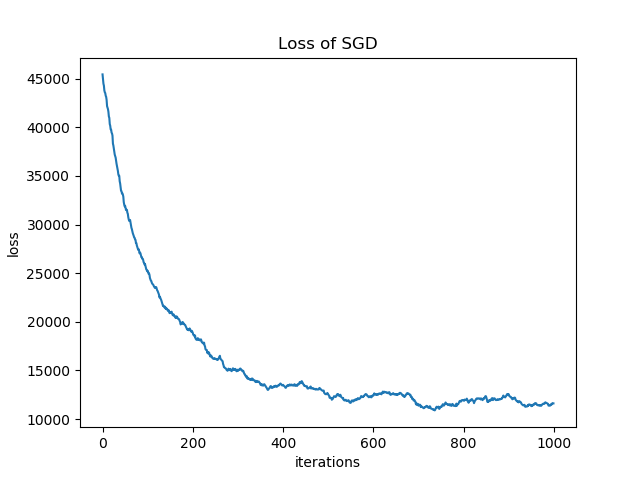
\includegraphics[width=\columnwidth]{sto_re.png}
		% Create a subtitle for the figure.
		\caption{stochastic gradient descent result}
		% Define the label of the figure. It's good to use 'fig:title', so you know that the label belongs to a figure.
		\label{fig4}
		\end{center}
	\end{figure}


\section{Conclusion}
	After the lab, I feel I have understood the knowledge that I have learned in the course better. I encountered many situations when I was completing my lab code. But as I consulted the slices and asked search engines again and again. I had a completely new understanding of machine learning. Many thanks to the professor and those graduate students who offered help.

% Your document ends here!
\end{document}
